\subsection{Blockschaltbild PCB}
Mit den nun bekannten Hauptbauteilen wurde zunächst ein Blockschaltbild erstellt, um die Signale zwischen den einzelnen Komponenten zu definieren. Dabei wurden für einige Komponenten bereits vordefiniert, da eine komplette Detailevaluation zu Zeitintensiv gewesen wäre. Die Überlegungen dazu sind nachfolgend kurz erläutert. Abbildung \ref{pic:blockschaltbild_pcb} zeigt das Blockschaltbild. 
\newpage
\begin{figure}[H]
	\centering
	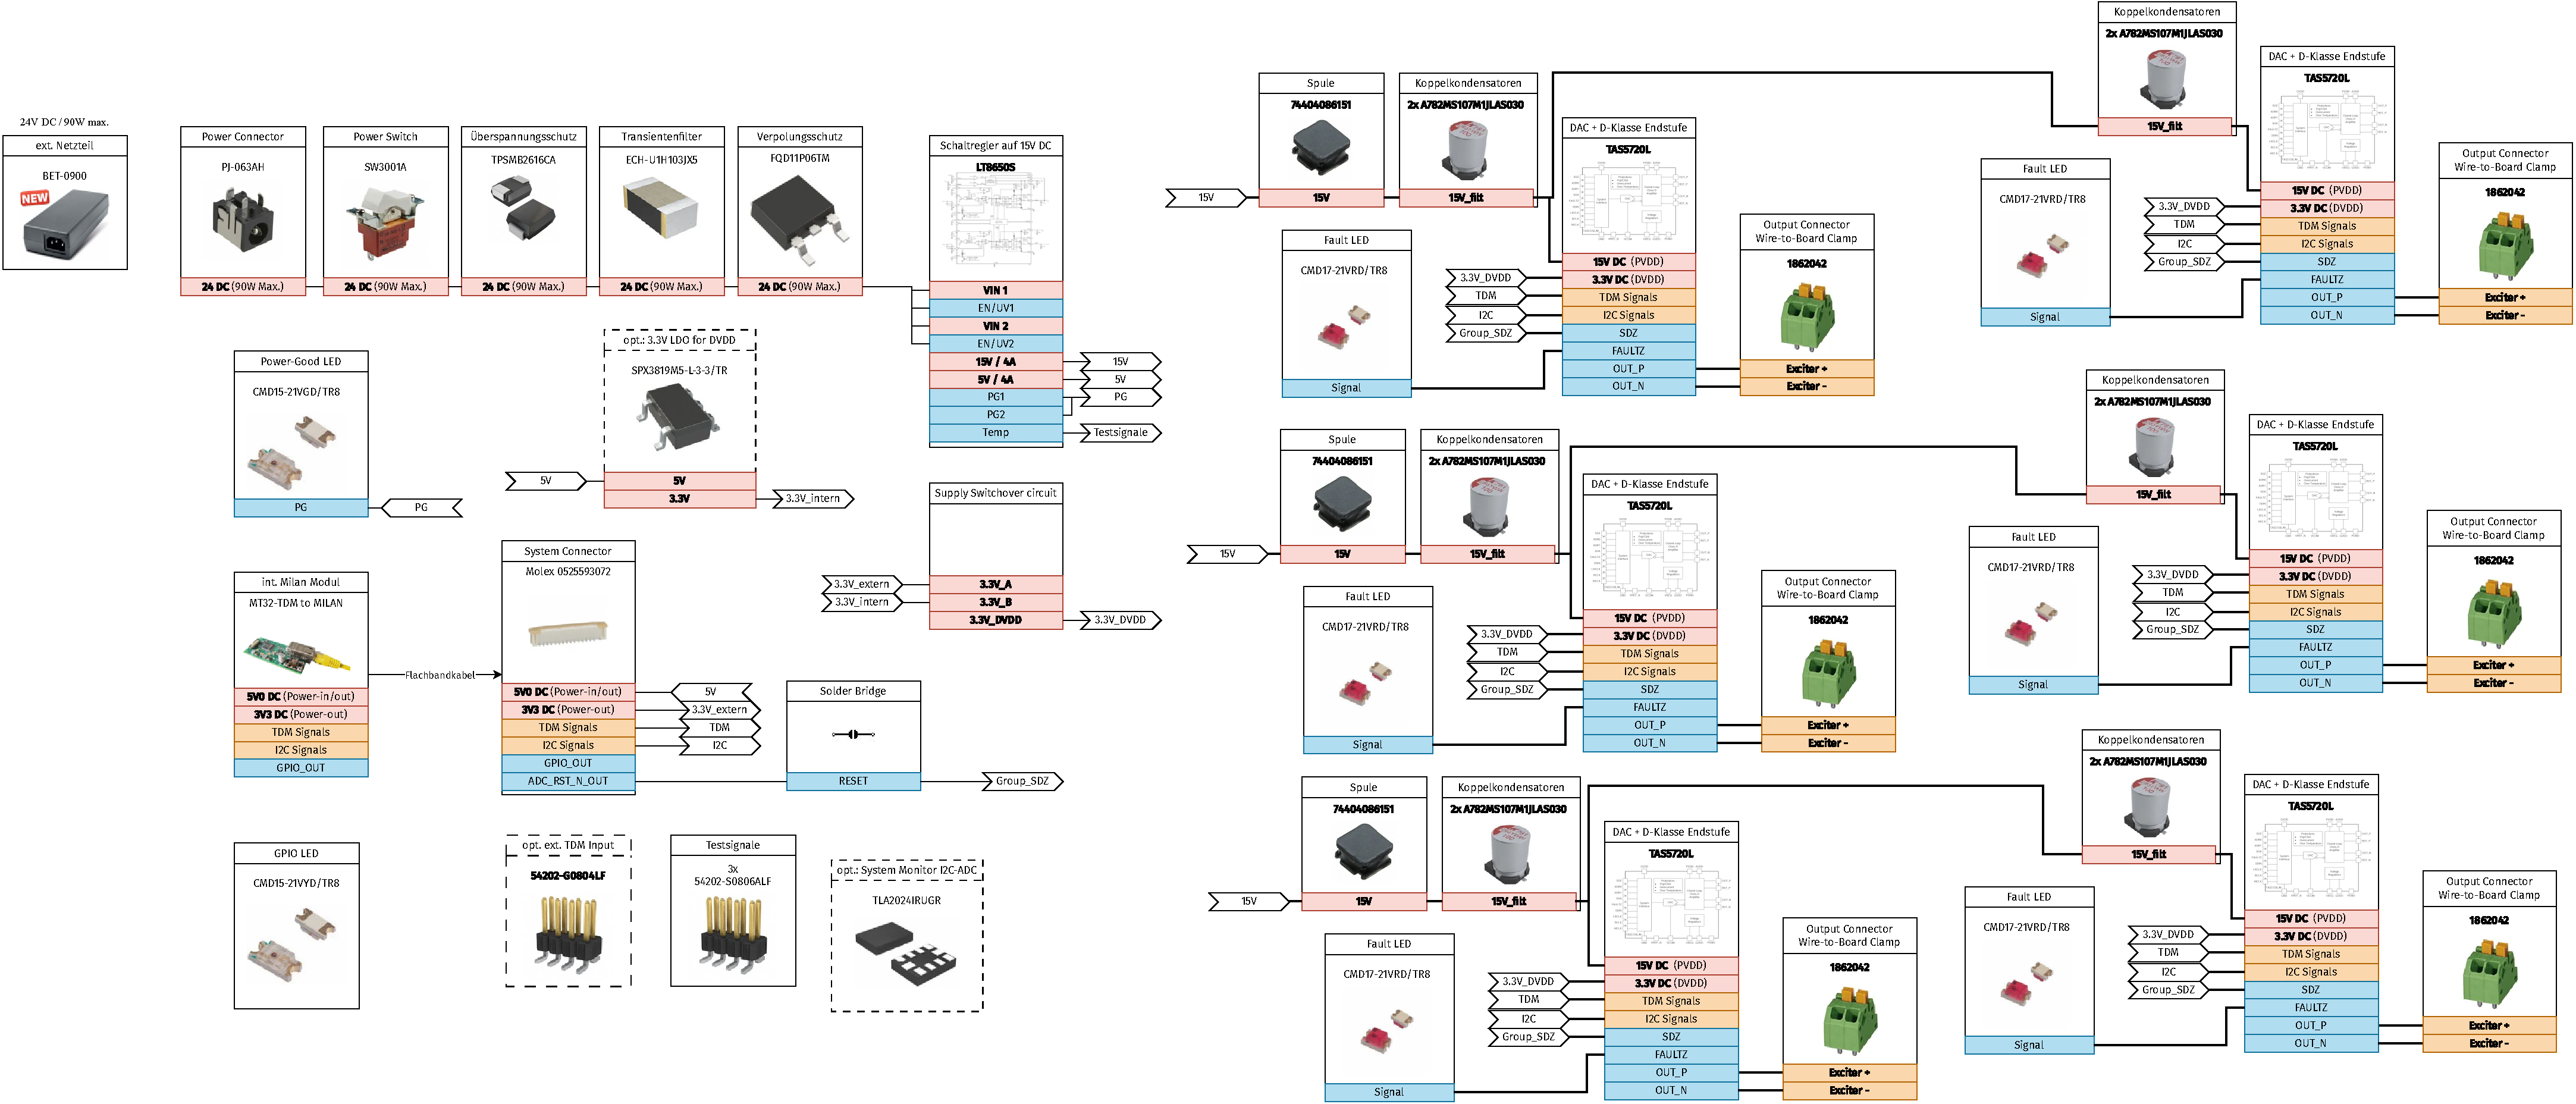
\includegraphics[width=\textheight - 1cm, angle=90]{pictures/blockschaltbild_pcb.pdf}
	\caption{Erster Entwurf des Blockschaltbildes}
	\label{pic:blockschaltbild_pcb}
\end{figure}